\flushcolsend
\clearpage
\appendix[Artifact description]


\subsection{Abstract}

Our research artifact consists of interactive Jupyter notebooks. The notebooks
enable users to replicate all experiments in the paper, evaluate results, and
plot figures.

\subsection{Description}

\subsubsection{Check-list (Artifact Meta Information)}

{\small
\begin{itemize}
  \item {\bf Run-time environment: }Ubuntu Linux and a web browser.
  \item {\bf Hardware: }Users with an NVIDIA GPU may enable CUDA support to
    speed up computation of experiments.
  \item {\bf Output: }Trained neural networks, predictive model evaluations,
    figures and tables from the paper.
  \item {\bf Experiment workflow: }Install and run Jupyter notebook server;
    interact with and observe results in web browser.
  \item {\bf Experiment customization: }Edit code and parameters in Jupyter
    notebooks.
  \item {\bf Publicly available?: }Yes, code and data. See:\\*
    \url{https://chriscummins.cc/pact17/}
  \end{itemize}
}

\subsubsection{How Delivered}

A publicly available git repository containing Jupyter notebooks and
experimental data.


\subsection{Installation}\label{subsec:installation}

See \url{https://chriscummins.cc/pact17/} for instructions. The \texttt{code}
directory contains the Jupyter notebooks. Following the build instructions
described in \texttt{code/README.md}, the full installation process is:

\begin{verbatim}
$ ./bootstrap.sh | bash
$ ./configure
$ make
\end{verbatim}


\subsection{Experiment Workflow}\label{subsec:workflow}

\begin{enumerate}
  \item Launch the Jupyter server using the command:\\*
  \texttt{make run}.
  \item In a web browser, navigate to:\\* \texttt{http://localhost:8000}.
  \item Select a Jupyter notebook to open it.
  \item Repeatedly press the \emph{play} button (tooltip is ``run cell, select
    below'') to step through each cell of the notebook.

  OR select ``Kernel'' $>$ ``Restart \& Run All'' from the menu to run all of
  the cells in order.
  \begin{figure}[H]
    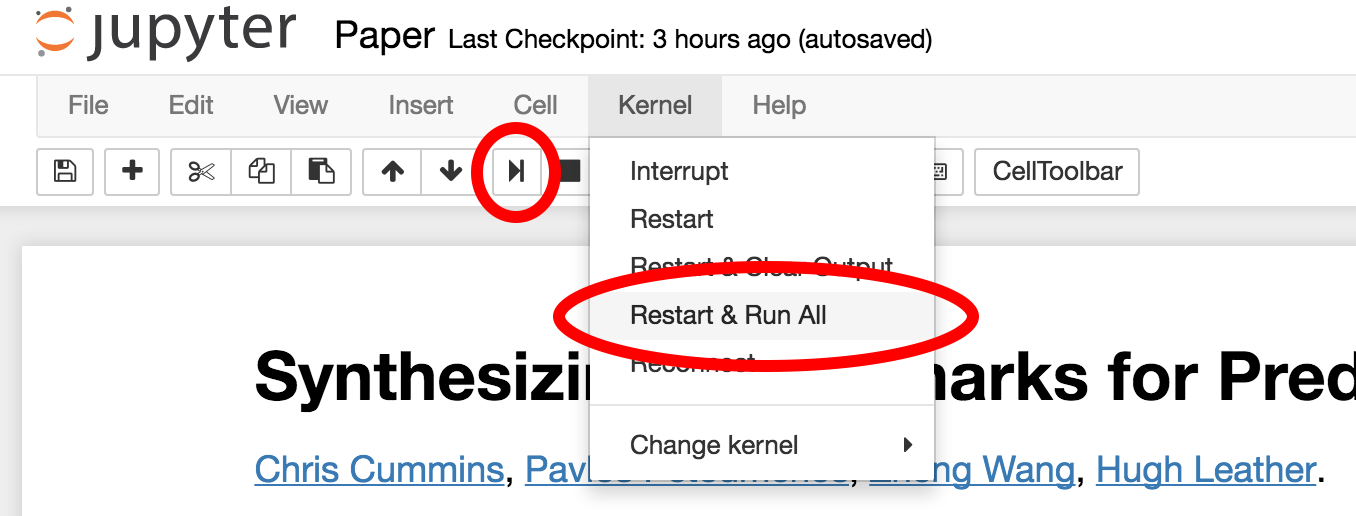
\includegraphics[width=\columnwidth]{img/jupyter}
  \end{figure}
\end{enumerate}


\subsection{Evaluation and Expected Result}

Code cells within Jupyter notebooks display their output inline, and may be
compared against the values in the paper. Expected results are described in text
cells.


\subsection{Experiment Customization}

The experiments are fully customizable. The Jupyter notebook can be edited ``on
the fly''. Simply type your changes into the cells and re-run them.

\noindent Note that some of the code cells depend on the values of prior cells,
so must be executed in sequence. Select ``Kernel'' $>$ ``Restart \& Run All''
from the menu to run all of the cells in order.


\subsection{Notes}
\noindent For more information about DeepTune, visit:

\url{https://chriscummins.cc/deeptune}

\noindent For more information about Artifact Evaluation, visit:

\url{http://cTuning.org/ae/submission-20170414.html}

% Fix rendering layout error introduced by flushend package:
\raggedend
